\chapter{SWID Generator}

\section{Requirements}

\subsection{Zweck}

Der SWID Generator soll ein kleines Programm für Linux-Systeme sein, welches aus
den Informationen in Paket Management Systemen SWID Tags generiert.

\subsection{Nichtfunktionale Anforderungen}

\begin{itemize}
		\item Als Implementationsprache wird Python verwendet.
		\item Es sollen möglichst wenig Abhängigkeiten zu Drittkomponenten wie
			Libraries/Frameworks entstehen.
    \item Die Software soll einfach zu installieren sein, beispielsweise durch
			Upload in den Python Package Index ($\rightarrow$ \texttt{pip install
			swid-generator}) oder durch Erstellen von \texttt{.deb}- und
			\texttt{.rpm}-Paketen.
    \item Als Quelle der Paketinformationen sollen Paketmanager wie DPKG und RPM
			verwendet werden.
\end{itemize}

\subsection{Use Cases}

Nachfolgend sind sind die identifizierten Use Cases für die Client Komponenten
des SWID-Generator aufgeführt.

Dabei werden die folgen drei Systemkomponenten berücksichtigt, welche
gegenseitig über die Standardeingabe und -ausgabe kommunizieren.

\vspace{1em}

\begin{figure}[H]
	\centering
	\definecolor{StrongswanColor}{RGB}{199,108,107}
\definecolor{GeneratorColor}{RGB}{116,143,204}
\definecolor{PkgMgrColor}{RGB}{227,225,107}

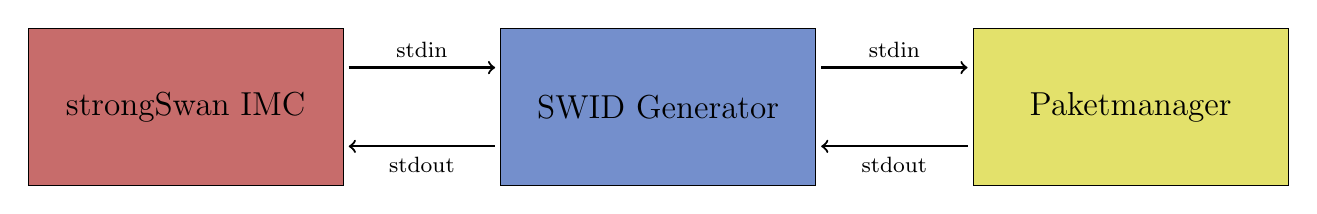
\begin{tikzpicture}[
		actor/.style={font=\large},
		communication/.style={thick, shorten <= 2pt, shorten >= 2pt, font=\footnotesize}
	]

	% Rectangles
	\filldraw[fill=StrongswanColor] (0, 0) rectangle node[actor] {strongSwan IMC} (4, 2);
	\filldraw[fill=GeneratorColor] (6, 0) rectangle node[actor] {SWID Generator} (10, 2);
	\filldraw[fill=PkgMgrColor] (12, 0) rectangle node[actor] {Paketmanager} (16, 2);

	% Arrows
	\draw[->, communication] (4, 1.5) -- node[above] {stdin} (6, 1.5);
	\draw[<-, communication] (4, 0.5) -- node[below] {stdout} (6, 0.5);
	\draw[->, communication] (10, 1.5) -- node[above] {stdin} (12, 1.5);
	\draw[<-, communication] (10, 0.5) -- node[below] {stdout} (12, 0.5);


\end{tikzpicture}

	\caption{SWID Generator: Systemkomponenten}
	\label{img:swid-generator-aktoren}
\end{figure}

\subsubsection{UC01: Erkennung des Paketmanagers}

\begin{tabularx}{\textwidth}{lX}
\hline 
\textbf{Actor} & strongSwan IMC \\ 
\hline
\textbf{Story} &
Der strongSwan IMC weiss nicht ob auf dem Zielsystem yum oder dpkg verwendet wird. Der swid Generator soll den verwendeten Paketmanager automatisch erkennen. \\
\hline 
\textbf{Standard Szenario} & 
Der SWID-Generator erkennt automatisch den System-Paketmanager und greift auf
dessen Datenbank zu. \\ 
\hline 
\textbf{Alternatives Szenario} &
Mittels optionalem Parameter kann der zu verwendende Packagemanager definiert
werden, die Autoerkennung wird dadurch übersteuert.
\end{tabularx} 

\paragraph{Standard Szenario}
Der SWID-Generator erkennt automatisch den System-Paketmanager und greift auf
dessen Datenbank zu.

\paragraph{Alternatives Szenario}
Mittels optionalem Parameter kann der zu verwendende Packagemanager definiert
werden, die Autoerkennung wird dadurch übersteuert.

\subsubsection{UC02: Standard SWID Generierung}

Die IMC Komponente kann via stdout des SWID-Generators XML Dokumente erhalten, welche Informationen über die zur Zeit installierte Software des Zielsystems beinhalten.
Das Format dieser XML Dokumente folgt dem ISO Draft 19770-2-5
Für jedes installierte Paket wird ein eigenes ein XML Dokument generiert.
Diese Dokumente bestehen im wesentlichen aus einem SoftwareIdentity-Tag als Root-Knoten und einem Entity-Tag als Kind-Knoten. Die Information findet sich in den entsprechenden Attributen.

\begin{minted}{xml}
<?xml version='1.0' encoding='UTF-8'?>
<SoftwareIdentity
    name="apparmor"
    uniqueId="Ubuntu_13.10-apparmor-2.8.0-0ubuntu31.1"
    version="2.8.0-0ubuntu31.1"
    versionScheme="alphanumeric"
    xmlns="http://standards.iso.org/iso/19770/-2/2014/schema.xsd">

    <Entity
        name="strongSwan"
        regid="regid.2004-03.org.strongswan"
        role="tagcreator" />
</SoftwareIdentity>
\end{minted}

\paragraph{Standard Szenario}
Die Attribute werden mit vordefinierten Standardwerten befüllt. Siehe Codelisting oben (TODO: referenz).

\paragraph{Alternatives Szenario}
Die Attribute können mittels optionalem Parametern spezifiziert werden.

\subsubsection{UC03: SWID Tag mit File Payload}
Mittels optionalem Parameter können die XML Dokumente mit einem Payload-Tag versehen werden, welcher für jedes Paket die darin enthaltenen Dateien auflistet.
TODO Beispiel

\subsubsection{UC04: Ausgabe der Dokumente}

\paragraph{Standard Szenario}
Der Benutzer möchte die XML Dokumente parsen. Dafür führt er den Generator mit
Default-Parametern aus. Standardmässig wird jedes XML Dokument auf einer einzelnen Zeile
mit Newlines getrennt ausgegeben.

\paragraph{Alternatives Szenario}
Der Benutzer möchte die Dokumente in menschenlesbarer Form ausgeben (pretty
print). Das steuert er über optionale Parameter. Diese Ausgabe der Tags ist dann
hierarchisch eingerückt um so die Lesbarkeit sicherzustellen.

\subsubsection{UC05: Ausgabe der Tag-ID's}
Der strongSwan IMC möchte nur Tag-ID's von den installierten Paketen erhalten. Bei Tag-ID's handelt es sich nicht um XML Dokumente, sondern einfache Strings im Format $regid\_uniqueID $. Diese sollen zeilengetrennt ($\backslash$n$\backslash$n) ausgegeben werden. Beispiel:\\
\begin{minted}{xml}
regid.2004-03.org.strongswan_fedora_19-64bit-NetworkManager-glib.i686-1:0.9.8.2-2.fc19

regid.2004-03.org.strongswan_fedora_19-64bit-bash.i686-4.2.45-1.fc19
\end{minted}
\paragraph{Alternatives Szenario}
Die Zeilentrennung der Strings kann mittels Parameter spezifiziert werden.

\subsubsection{UC06: Anfordern bestimmter SWID Tags}
Der strongSwan IMC möchte nur SWID Tags eines bestimmten Paketes erhalten.
Mittels Parameter kann dem Generator eine Wildcard/Filterwert angegeben werden, um so targeted Requests ausführen zukönnen.


\section{Paketverwaltungen}

\subsubsection{DPKG}

DPKG\footnote{\url{https://alioth.debian.org/projects/dpkg}} (Abkürzung für
\textit{Debian Package}) ist die Basis der Paketverwaltung in Debian und in
verwandten Distributionen wie Ubuntu. DPKG verwaltet unter anderem alle
installierten Software-Pakete inklusive Meta-Informationen. Diese Paketliste
kann mit \texttt{dpkg-query} abgefragt werden.

\paragraph{Installierte Pakete abfragen} \hspace{0pt} \\

\noindent Mit \texttt{dpkg ---show} wird eine Liste aller installierter Pakete
ausgegeben, ein Paket pro Zeile. Um die Ausgabe zu personalisieren kann das
\texttt{---showformat} Flag verwendet werden. Im Falle des swidGenerators
ist folgendes Format ideal:

\begin{bashcode}
dpkg-query --show --showformat='${Package}\t${Version}\t${Status}\n'
\end{bashcode}

\noindent Hierbei ist noch anzumerken, dass entfernte DPKG Pakete einen sogenannten RC Status haben können. Dieser liegt vor, wenn ein Paket deinstalliert, aber die Konfigurationsdateien auf dem System belassen wurden. Die \texttt{---show} Option liefert auch diese Pakete . Dieser Der Zustand im Status Feld als \texttt{deinstall ok config-files} ersichtlich, entsprechende Pakete können so nachträglich im swidGenerator noch gefiltert werden.
\paragraph{Paket-Dateien abfragen} \hspace{0pt} \\

\noindent Um die zu einem Paket zugehörigen Dateien abzufragen, kann das
\texttt{---listfiles} Flag verwendet werden:

\begin{bashcode}
dpkg-query --listfiles <package-name>
\end{bashcode}

\paragraph{Datei-Hashes abfragen} \hspace{0pt} \\

\noindent Es besteht die Möglichkeit, aus DPKG MD5-Hashes der Dateien abzufragen. Weitere
Hash-Algorithmen (beispielsweise SHA) sind nicht verfügbar.


\subsubsection{RPM}

RPM\footnote{\url{https://rpm.org}} (Abkürzung für
\textit{Red Hat Package Manager}) ist die Standardpaketverwaltung für Red Hat Systeme sowie zahlreichen verwandten Distributionen wie SUSE, Mandriva und Fedora.

\paragraph{Installierte Pakete abfragen} \hspace{0pt} \\

\noindent Ähnlich wie bei dpkg können alle auf dem System vorhandenen Pakete abgefragt werden. Die Ausgabe kann auch via Format String personalisiert werden. Für den swidGenerator ist folgendes Format ideal:

\begin{bashcode}
rpm -qa --queryformat %{name}\t%{version}-%{release}
\end{bashcode}

\paragraph{Paket-Dateien abfragen} \hspace{0pt} \\

\noindent Um die zu einem Paket zugehörigen Dateien abzufragen, können die Parameter \texttt{--ql} verwendet werden:

\begin{bashcode}
rpm -ql <package-name>
\end{bashcode}

\noindent TODO
